
%% bare_conf.tex
%% V1.3
%% 2007/01/11
%% by Michael Shell
%% See:
%% http://www.michaelshell.org/
%% for current contact information.
%%
%% This is a skeleton file demonstrating the use of IEEEtran.cls
%% (requires IEEEtran.cls version 1.7 or later) with an IEEE conference paper.
%%
%% Support sites:
%% http://www.michaelshell.org/tex/ieeetran/
%% http://www.ctan.org/tex-archive/macros/latex/contrib/IEEEtran/
%% and
%% http://www.ieee.org/

%%*************************************************************************
%% Legal Notice:
%% This code is offered as-is without any warranty either expressed or
%% implied; without even the implied warranty of MERCHANTABILITY or
%% FITNESS FOR A PARTICULAR PURPOSE! 
%% User assumes all risk.
%% In no event shall IEEE or any contributor to this code be liable for
%% any damages or losses, including, but not limited to, incidental,
%% consequential, or any other damages, resulting from the use or misuse
%% of any information contained here.
%%
%% All comments are the opinions of their respective authors and are not
%% necessarily endorsed by the IEEE.
%%
%% This work is distributed under the LaTeX Project Public License (LPPL)
%% ( http://www.latex-project.org/ ) version 1.3, and may be freely used,
%% distributed and modified. A copy of the LPPL, version 1.3, is included
%% in the base LaTeX documentation of all distributions of LaTeX released
%% 2003/12/01 or later.
%% Retain all contribution notices and credits.
%% ** Modified files should be clearly indicated as such, including  **
%% ** renaming them and changing author support contact information. **
%%
%% File list of work: IEEEtran.cls, IEEEtran_HOWTO.pdf, bare_adv.tex,
%%                    bare_conf.tex, bare_jrnl.tex, bare_jrnl_compsoc.tex
%%*************************************************************************

% *** Authors should verify (and, if needed, correct) their LaTeX system  ***
% *** with the testflow diagnostic prior to trusting their LaTeX platform ***
% *** with production work. IEEE's font choices can trigger bugs that do  ***
% *** not appear when using other class files.                            ***
% The testflow support page is at:
% http://www.michaelshell.org/tex/testflow/



% Note that the a4paper option is mainly intended so that authors in
% countries using A4 can easily print to A4 and see how their papers will
% look in print - the typesetting of the document will not typically be
% affected with changes in paper size (but the bottom and side margins will).
% Use the testflow package mentioned above to verify correct handling of
% both paper sizes by the user's LaTeX system.
%
% Also note that the "draftcls" or "draftclsnofoot", not "draft", option
% should be used if it is desired that the figures are to be displayed in
% draft mode.
%
\documentclass[conference]{IEEEtran}
\usepackage{blindtext, graphicx}
\graphicspath{ {C:/Users/Frazierhuo/Desktop/Sentiment_Analysis/sentiment_analysis/IEEE Conference} }
% Add the compsoc option for Computer Society conferences.
%
% If IEEEtran.cls has not been installed into the LaTeX system files,
% manually specify the path to it like:
% \documentclass[conference]{../sty/IEEEtran}





% Some very useful LaTeX packages include:
% (uncomment the ones you want to load)


% *** MISC UTILITY PACKAGES ***
%
%\usepackage{ifpdf}
% Heiko Oberdiek's ifpdf.sty is very useful if you need conditional
% compilation based on whether the output is pdf or dvi.
% usage:
% \ifpdf
%   % pdf code
% \else
%   % dvi code
% \fi
% The latest version of ifpdf.sty can be obtained from:
% http://www.ctan.org/tex-archive/macros/latex/contrib/oberdiek/
% Also, note that IEEEtran.cls V1.7 and later provides a builtin
% \ifCLASSINFOpdf conditional that works the same way.
% When switching from latex to pdflatex and vice-versa, the compiler may
% have to be run twice to clear warning/error messages.






% *** CITATION PACKAGES ***
%
%\usepackage{cite}
% cite.sty was written by Donald Arseneau
% V1.6 and later of IEEEtran pre-defines the format of the cite.sty package
% \cite{} output to follow that of IEEE. Loading the cite package will
% result in citation numbers being automatically sorted and properly
% "compressed/ranged". e.g., [1], [9], [2], [7], [5], [6] without using
% cite.sty will become [1], [2], [5]--[7], [9] using cite.sty. cite.sty's
% \cite will automatically add leading space, if needed. Use cite.sty's
% noadjust option (cite.sty V3.8 and later) if you want to turn this off.
% cite.sty is already installed on most LaTeX systems. Be sure and use
% version 4.0 (2003-05-27) and later if using hyperref.sty. cite.sty does
% not currently provide for hyperlinked citations.
% The latest version can be obtained at:
% http://www.ctan.org/tex-archive/macros/latex/contrib/cite/
% The documentation is contained in the cite.sty file itself.






% *** GRAPHICS RELATED PACKAGES ***
%
\ifCLASSINFOpdf
  % \usepackage[pdftex]{graphicx}
  % declare the path(s) where your graphic files are
  % \graphicspath{{../pdf/}{../jpeg/}}
  % and their extensions so you won't have to specify these with
  % every instance of \includegraphics
  % \DeclareGraphicsExtensions{.pdf,.jpeg,.png}
\else
  % or other class option (dvipsone, dvipdf, if not using dvips). graphicx
  % will default to the driver specified in the system graphics.cfg if no
  % driver is specified.
  % \usepackage[dvips]{graphicx}
  % declare the path(s) where your graphic files are
  % \graphicspath{{../eps/}}
  % and their extensions so you won't have to specify these with
  % every instance of \includegraphics
  % \DeclareGraphicsExtensions{.eps}
\fi
% graphicx was written by David Carlisle and Sebastian Rahtz. It is
% required if you want graphics, photos, etc. graphicx.sty is already
% installed on most LaTeX systems. The latest version and documentation can
% be obtained at: 
% http://www.ctan.org/tex-archive/macros/latex/required/graphics/
% Another good source of documentation is "Using Imported Graphics in
% LaTeX2e" by Keith Reckdahl which can be found as epslatex.ps or
% epslatex.pdf at: http://www.ctan.org/tex-archive/info/
%
% latex, and pdflatex in dvi mode, support graphics in encapsulated
% postscript (.eps) format. pdflatex in pdf mode supports graphics
% in .pdf, .jpeg, .png and .mps (metapost) formats. Users should ensure
% that all non-photo figures use a vector format (.eps, .pdf, .mps) and
% not a bitmapped formats (.jpeg, .png). IEEE frowns on bitmapped formats
% which can result in "jaggedy"/blurry rendering of lines and letters as
% well as large increases in file sizes.
%
% You can find documentation about the pdfTeX application at:
% http://www.tug.org/applications/pdftex





% *** MATH PACKAGES ***
%
%\usepackage[cmex10]{amsmath}
% A popular package from the American Mathematical Society that provides
% many useful and powerful commands for dealing with mathematics. If using
% it, be sure to load this package with the cmex10 option to ensure that
% only type 1 fonts will utilized at all point sizes. Without this option,
% it is possible that some math symbols, particularly those within
% footnotes, will be rendered in bitmap form which will result in a
% document that can not be IEEE Xplore compliant!
%
% Also, note that the amsmath package sets \interdisplaylinepenalty to 10000
% thus preventing page breaks from occurring within multiline equations. Use:
%\interdisplaylinepenalty=2500
% after loading amsmath to restore such page breaks as IEEEtran.cls normally
% does. amsmath.sty is already installed on most LaTeX systems. The latest
% version and documentation can be obtained at:
% http://www.ctan.org/tex-archive/macros/latex/required/amslatex/math/





% *** SPECIALIZED LIST PACKAGES ***
%
%\usepackage{algorithmic}
% algorithmic.sty was written by Peter Williams and Rogerio Brito.
% This package provides an algorithmic environment fo describing algorithms.
% You can use the algorithmic environment in-text or within a figure
% environment to provide for a floating algorithm. Do NOT use the algorithm
% floating environment provided by algorithm.sty (by the same authors) or
% algorithm2e.sty (by Christophe Fiorio) as IEEE does not use dedicated
% algorithm float types and packages that provide these will not provide
% correct IEEE style captions. The latest version and documentation of
% algorithmic.sty can be obtained at:
% http://www.ctan.org/tex-archive/macros/latex/contrib/algorithms/
% There is also a support site at:
% http://algorithms.berlios.de/index.html
% Also of interest may be the (relatively newer and more customizable)
% algorithmicx.sty package by Szasz Janos:
% http://www.ctan.org/tex-archive/macros/latex/contrib/algorithmicx/




% *** ALIGNMENT PACKAGES ***
%
%\usepackage{array}
% Frank Mittelbach's and David Carlisle's array.sty patches and improves
% the standard LaTeX2e array and tabular environments to provide better
% appearance and additional user controls. As the default LaTeX2e table
% generation code is lacking to the point of almost being broken with
% respect to the quality of the end results, all users are strongly
% advised to use an enhanced (at the very least that provided by array.sty)
% set of table tools. array.sty is already installed on most systems. The
% latest version and documentation can be obtained at:
% http://www.ctan.org/tex-archive/macros/latex/required/tools/


%\usepackage{mdwmath}
%\usepackage{mdwtab}
% Also highly recommended is Mark Wooding's extremely powerful MDW tools,
% especially mdwmath.sty and mdwtab.sty which are used to format equations
% and tables, respectively. The MDWtools set is already installed on most
% LaTeX systems. The lastest version and documentation is available at:
% http://www.ctan.org/tex-archive/macros/latex/contrib/mdwtools/


% IEEEtran contains the IEEEeqnarray family of commands that can be used to
% generate multiline equations as well as matrices, tables, etc., of high
% quality.


%\usepackage{eqparbox}
% Also of notable interest is Scott Pakin's eqparbox package for creating
% (automatically sized) equal width boxes - aka "natural width parboxes".
% Available at:
% http://www.ctan.org/tex-archive/macros/latex/contrib/eqparbox/





% *** SUBFIGURE PACKAGES ***
%\usepackage[tight,footnotesize]{subfigure}
% subfigure.sty was written by Steven Douglas Cochran. This package makes it
% easy to put subfigures in your figures. e.g., "Figure 1a and 1b". For IEEE
% work, it is a good idea to load it with the tight package option to reduce
% the amount of white space around the subfigures. subfigure.sty is already
% installed on most LaTeX systems. The latest version and documentation can
% be obtained at:
% http://www.ctan.org/tex-archive/obsolete/macros/latex/contrib/subfigure/
% subfigure.sty has been superceeded by subfig.sty.



%\usepackage[caption=false]{caption}
%\usepackage[font=footnotesize]{subfig}
% subfig.sty, also written by Steven Douglas Cochran, is the modern
% replacement for subfigure.sty. However, subfig.sty requires and
% automatically loads Axel Sommerfeldt's caption.sty which will override
% IEEEtran.cls handling of captions and this will result in nonIEEE style
% figure/table captions. To prevent this problem, be sure and preload
% caption.sty with its "caption=false" package option. This is will preserve
% IEEEtran.cls handing of captions. Version 1.3 (2005/06/28) and later 
% (recommended due to many improvements over 1.2) of subfig.sty supports
% the caption=false option directly:
%\usepackage[caption=false,font=footnotesize]{subfig}
%
% The latest version and documentation can be obtained at:
% http://www.ctan.org/tex-archive/macros/latex/contrib/subfig/
% The latest version and documentation of caption.sty can be obtained at:
% http://www.ctan.org/tex-archive/macros/latex/contrib/caption/




% *** FLOAT PACKAGES ***
%
%\usepackage{fixltx2e}
% fixltx2e, the successor to the earlier fix2col.sty, was written by
% Frank Mittelbach and David Carlisle. This package corrects a few problems
% in the LaTeX2e kernel, the most notable of which is that in current
% LaTeX2e releases, the ordering of single and double column floats is not
% guaranteed to be preserved. Thus, an unpatched LaTeX2e can allow a
% single column figure to be placed prior to an earlier double column
% figure. The latest version and documentation can be found at:
% http://www.ctan.org/tex-archive/macros/latex/base/



%\usepackage{stfloats}
% stfloats.sty was written by Sigitas Tolusis. This package gives LaTeX2e
% the ability to do double column floats at the bottom of the page as well
% as the top. (e.g., "\begin{figure*}[!b]" is not normally possible in
% LaTeX2e). It also provides a command:
%\fnbelowfloat
% to enable the placement of footnotes below bottom floats (the standard
% LaTeX2e kernel puts them above bottom floats). This is an invasive package
% which rewrites many portions of the LaTeX2e float routines. It may not work
% with other packages that modify the LaTeX2e float routines. The latest
% version and documentation can be obtained at:
% http://www.ctan.org/tex-archive/macros/latex/contrib/sttools/
% Documentation is contained in the stfloats.sty comments as well as in the
% presfull.pdf file. Do not use the stfloats baselinefloat ability as IEEE
% does not allow \baselineskip to stretch. Authors submitting work to the
% IEEE should note that IEEE rarely uses double column equations and
% that authors should try to avoid such use. Do not be tempted to use the
% cuted.sty or midfloat.sty packages (also by Sigitas Tolusis) as IEEE does
% not format its papers in such ways.





% *** PDF, URL AND HYPERLINK PACKAGES ***
%
%\usepackage{url}
% url.sty was written by Donald Arseneau. It provides better support for
% handling and breaking URLs. url.sty is already installed on most LaTeX
% systems. The latest version can be obtained at:
% http://www.ctan.org/tex-archive/macros/latex/contrib/misc/
% Read the url.sty source comments for usage information. Basically,
% \url{my_url_here}.





% *** Do not adjust lengths that control margins, column widths, etc. ***
% *** Do not use packages that alter fonts (such as pslatex).         ***
% There should be no need to do such things with IEEEtran.cls V1.6 and later.
% (Unless specifically asked to do so by the journal or conference you plan
% to submit to, of course. )


% correct bad hyphenation here
\hyphenation{op-tical net-works semi-conduc-tor}


\begin{document}
%
% paper title
% can use linebreaks \\ within to get better formatting as desired
\title{Sentiment analysis on Twitter using semeval 2016 data}


% author names and affiliations
% use a multiple column layout for up to three different
% affiliations
\author{\IEEEauthorblockN{Zepeng Huo}
\IEEEauthorblockA{Department of Computer\\Science and Engineering\\
Texas A\&M University\\
Email: Guangzhou92@tamu.edu}
\and
\IEEEauthorblockN{Pradnyil Sranjay}
\IEEEauthorblockA{Department of Industrial\\and Systems Engineering\\
Texas A\&M University\\
Email: pradnyil@tamu.edu}
}

% conference papers do not typically use \thanks and this command
% is locked out in conference mode. If really needed, such as for
% the acknowledgment of grants, issue a \IEEEoverridecommandlockouts
% after \documentclass

% for over three affiliations, or if they all won't fit within the width
% of the page, use this alternative format:
% 
%\author{\IEEEauthorblockN{Michael Shell\IEEEauthorrefmark{1},
%Homer Simpson\IEEEauthorrefmark{2},
%James Kirk\IEEEauthorrefmark{3}, 
%Montgomery Scott\IEEEauthorrefmark{3} and
%Eldon Tyrell\IEEEauthorrefmark{4}}
%\IEEEauthorblockA{\IEEEauthorrefmark{1}School of Electrical and Computer Engineering\\
%Georgia Institute of Technology,
%Atlanta, Georgia 30332--0250\\ Email: see http://www.michaelshell.org/contact.html}
%\IEEEauthorblockA{\IEEEauthorrefmark{2}Twentieth Century Fox, Springfield, USA\\
%Email: homer@thesimpsons.com}
%\IEEEauthorblockA{\IEEEauthorrefmark{3}Starfleet Academy, San Francisco, California 96678-2391\\
%Telephone: (800) 555--1212, Fax: (888) 555--1212}
%\IEEEauthorblockA{\IEEEauthorrefmark{4}Tyrell Inc., 123 Replicant Street, Los Angeles, California 90210--4321}}




% use for special paper notices
%\IEEEspecialpapernotice{(Invited Paper)}




% make the title area
\maketitle


\begin{abstract}
%\boldmath
Sentiment analysis is getting popular on social media. In this paper, we propose a method to classify the emotion valence of a given tweet. The whole framework can be separated as two parts: first, we cluster the similar tweets based on the fact that all data of semeval-2016 are collected from specific topics. And the topic can be distinguished as three different parts. Based on the result of clustering, we feed the tweet into the Tensorflow network to classify.
\end{abstract}
% IEEEtran.cls defaults to using nonbold math in the Abstract.
% This preserves the distinction between vectors and scalars. However,
% if the journal you are submitting to favors bold math in the abstract,
% then you can use LaTeX's standard command \boldmath at the very start
% of the abstract to achieve this. Many IEEE journals frown on math
% in the abstract anyway.

% Note that keywords are not normally used for peerreview papers.
\begin{IEEEkeywords}
Social Media, Sentiment Analysis, Clustering, Neural Network, Tensorflow.
\end{IEEEkeywords}






% For peer review papers, you can put extra information on the cover
% page as needed:
% \ifCLASSOPTIONpeerreview
% \begin{center} \bfseries EDICS Category: 3-BBND \end{center}
% \fi
%
% For peerreview papers, this IEEEtran command inserts a page break and
% creates the second title. It will be ignored for other modes.
\IEEEpeerreviewmaketitle

\section{Introduction}
The problem of sentiment classification is not a new one and now nor is that of twitter sentiment classification. The first appearance in the Semeval tasks was in 2013 and this particular task has had a rerun ever since. But over the years the approach and methodology used in for this task has undergone a lot of changes. As noted by HLTCOE, JHU. Et all (2013). in the review of the 2013 team participants all the teams used a supervised learning approach to the task by employing human generated features to feed to a classification algorithm. In the most recent review of the same task by Nakov, Preslav, 2016.et all, the most popular systems used are the deep neural networks like convolution neural networks and recurrent neural networks. The trend of shifting away from human trained features to a more semi supervised technique was the motivation for the use of our approach to the problem. 



\section{Task and Problem}
In Semeval 2016 competition task 4, Twitter sentiment analysis, we need to find out a way to classify sentiment of tweets. The data they provided is of two parts, training set and testing set. Each dataset consists of a couple thousand tweets and each tweets are labeled as either 'positive' or 'negative'. There are 5 subtasks and we only focus on the first one, binary classification. The data are collected by topics. Each topic has a couple hundred tweets. In other subtasks, the data comes with another label called 'topic'. And these subtasks aim to classify sentiment of tweets based on topics. However, in the subtask, we don't have this label. But it gives us idea that these tweets are distinguishable by topics. Thus, in order to make use of topic relatedness, we cluster the tweets in three broad categories. In each cluster, we have a particular classification model to classify that category. As for classification model, we use the Tensorflow neural network. The reason we want to use this model is because it's robust to noisy input but also sensitive to distinguishable text which can carry emotional expression.

\section{High-level description of approach}
We will have two tasks. The first task was training a model using all the data in the dataset irrespective of the cluster it belongs to. This model does a binary classification of the input tweets into positive and negative tweets. For this problem we used the SVM as a baseline and then a convolution neural network was used to compare the two models.
\\ \indent
In the second task, we first cluster the data into the 3 relevant clusters and then we feed the clustered tweets as input to the CNN model. We built a simple single layer CNN to handle the classification task. The tweets  In the model tuning process, the data input type to the model and the model parameters  were tuned. We will take a closer look at the neural network in the next section.
\\ \indent
Before the classification, we need to tokenize all the tweets in Twitter context. This step is necessary because some expression may be unique on social media like Twitter and thus carry specific emotion. For example, the emoticon ':)' means happy or smiley, and it is highly likely related to positive sentiment. But if we use normal tokenization method, it may separate it as ':' and ')', so it loses its original meaning. The tokenization method we use is twokenize. It's specific to Twitter and make every token intact, without adding or losing meanings. After tokenization, we can feed each tweets into a binary classification.
Since we use two steps to classify each tweet, we'll introduce the problems we tackled on each step.
\\ \indent
\begin{figure}[h]
\centering
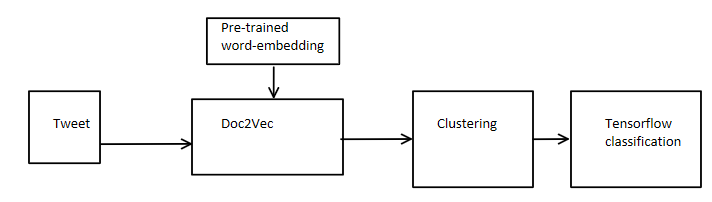
\includegraphics[width=0.5\textwidth]{Capture(2)}
\caption{Framework of 2-step classification}

\end{figure}
As for clustering, we want to make use of the hidden information under the data provided by Semeval-2106. Even though this subtask doesn't require to classify topics, we still want to have related tweets to be classified when they share similar topics. Normally, other sentiment analysis always feed all the texts into one classification model. But sometimes, some texts are harder than others to classify, for example, two tweets talk about the same topic and thus likely use similar wording. Distinguishing the nuance between them is harder than other tweets. So the intuition is that we need to use a powerful classification model to distinguish the tweets that are similar, which are thus harder to classify. So we use a pre-trained word embedding to make the underlying topic in each tweet more salient. The way pre-trained word embedding was created is to cluster similar tweets sharing similar topics. Therefore, each word vector representing one original English word is similar to another word vector carrying a word with meaning close to the first one. At the original data in other subtasks, the dataset has 60 topics. But most of them are highly related, for example, 'apple' and 'apple watch', 'Donald Trump' and 'Hillary'. Usually, when people are talking about this similar topics, they tend to use similar words carrying similar emotions. But when they talk about other topics, this words can express opposite sentiment, thus making the classification give unsatisfactory results. We want to classify similar tweets in one topic-specific classification. We chose the size of clustering categories as 3. The number of categories is not too big, such as originally 60, making the model underfitted. Nor it's not too small to make the less related tweets have fallen into same cluster.

% needed in second column of first page if using \IEEEpubid
%\IEEEpubidadjcol

% An example of a floating figure using the graphicx package.
% Note that \label must occur AFTER (or within) \caption.
% For figures, \caption should occur after the \includegraphics.
% Note that IEEEtran v1.7 and later has special internal code that
% is designed to preserve the operation of \label within \caption
% even when the captionsoff option is in effect. However, because
% of issues like this, it may be the safest practice to put all your
% \label just after \caption rather than within \caption{}.
%
% Reminder: the "draftcls" or "draftclsnofoot", not "draft", class
% option should be used if it is desired that the figures are to be
% displayed while in draft mode.
%
%\begin{figure}[!t]
%\centering
%\includegraphics[width=2.5in]{myfigure}
% where an .eps filename suffix will be assumed under latex, 
% and a .pdf suffix will be assumed for pdflatex; or what has been declared
% via \DeclareGraphicsExtensions.
%\caption{Simulation Results}
%\label{fig_sim}
%\end{figure}

% Note that IEEE typically puts floats only at the top, even when this
% results in a large percentage of a column being occupied by floats.


% An example of a double column floating figure using two subfigures.
% (The subfig.sty package must be loaded for this to work.)
% The subfigure \label commands are set within each subfloat command, the
% \label for the overall figure must come after \caption.
% \hfil must be used as a separator to get equal spacing.
% The subfigure.sty package works much the same way, except \subfigure is
% used instead of \subfloat.
%
%\begin{figure*}[!t]
%\centerline{\subfloat[Case I]\includegraphics[width=2.5in]{subfigcase1}%
%\label{fig_first_case}}
%\hfil
%\subfloat[Case II]{\includegraphics[width=2.5in]{subfigcase2}%
%\label{fig_second_case}}}
%\caption{Simulation results}
%\label{fig_sim}
%\end{figure*}
%
% Note that often IEEE papers with subfigures do not employ subfigure
% captions (using the optional argument to \subfloat), but instead will
% reference/describe all of them (a), (b), etc., within the main caption.


% An example of a floating table. Note that, for IEEE style tables, the 
% \caption command should come BEFORE the table. Table text will default to
% \footnotesize as IEEE normally uses this smaller font for tables.
% The \label must come after \caption as always.
%
%\begin{table}[!t]
%% increase table row spacing, adjust to taste
%\renewcommand{\arraystretch}{1.3}
% if using array.sty, it might be a good idea to tweak the value of
% \extrarowheight as needed to properly center the text within the cells
%\caption{An Example of a Table}
%\label{table_example}
%\centering
%% Some packages, such as MDW tools, offer better commands for making tables
%% than the plain LaTeX2e tabular which is used here.
%\begin{tabular}{|c||c|}
%\hline
%One & Two\\
%\hline
%Three & Four\\
%\hline
%\end{tabular}
%\end{table}


% Note that IEEE does not put floats in the very first column - or typically
% anywhere on the first page for that matter. Also, in-text middle ("here")
% positioning is not used. Most IEEE journals use top floats exclusively.
% Note that, LaTeX2e, unlike IEEE journals, places footnotes above bottom
% floats. This can be corrected via the \fnbelowfloat command of the
% stfloats package.

\section{Specific System Implementations}
In the part of clustering, we have our novelty in the system. First, as for converting the tweet into a mathematical representation, most common way is to use bag of words and word embedding. Then the whole tweet is concatenation or averaged vector of word embedding. These methods have problems of either making tweets vectors too long or losing lots of latent information by averaging word vectors. In our system, we use Doc2Vec. It can learn the vector of one sentence of one document by going through the corpus we provide. It then simultaneously learns the word vector in each tweet and the document vector of that tweet. The words appearing in similar context will likely have similar vector representation. The tweets consisting of similar word vectors will have similar document vectors. Thus, the Doc2Vec can preserve the original information in the tweet at the greatest extend and also avoid increasing the tweet vector dimension unnecessarily. Both the time complexity and space complexity can come to a balance.
\\ \indent
Since the dataset Semeval provides is relatively small (up to 6000 tweets for training), we may have the problem of overfitting the data thus making the noisy input contaminate the model. For example, if some of the tweets are using sarcasm and making positive adjectives carrying negative emotions. If we only train on these tweets, it's highly likely that similar positive words will be classified negative in other tweets, even though these tweets didn't use sarcasm. In the light of this, we propose a method to make the vector initialization closer to a well-established understanding of English words in Twitter. By initializing the word embedding using pre-trained word vectors, the document vector is more likely to come to a optimum. For the pre-trained word embedding, we used the library called Global Vectors for Word Representation (GloVe). The pre-trained word vectors are trained on 2 billion tweets, ending having 27 billion tokens and 1.2 million vocabulary. After feeding pre-trained word embedding into the Doc2Vec model, we make our model carry more well-known usage of English words in Twitter. In this way, some noisy input from the training set we provide the classification model may be alleviated by giving each word the meaning all users on Twitter can easily agree on.
\\ \indent
After converting each tweet into a vector, we start clustering the tweets into three categories we discussed before. The cluster method we used is k-means. It can cluster most similar vectors together and make different vectors far away from each other. Based on the dimensionality of the vector space, 300, k-means performs well in time complexity.
\\ \indent
When finishing clustering, each tweet will be assigned a index indicating which cluster it belongs to. Then, we feed these tweet into the classification model specific to that topic category.
\\ \indent
As for classification part we trained a simple single layer CNN which is on top of the vectorized word embeddings. This model is a takes in the tweets as input, and cleans the tokenizes the tweets using the twokenize tweet tokenizer. The next step is the padding of the all the tweets in the data set. Due to the way a CNN is structured all the input data to the model needs to be of the same dimensional form. This is achieved by padding all the tweets to the length of the longest tweet in the dataset which was 38 tokens long. The character limit on twitter of 144 characters helps to keep in check the issues of loosing data information due to excessive padding. These are then suitably converted to matrices first in by just using a bag of words encoding. Let us look into the details of the model In many of the cases the choice of the hyper-parameters used and the implementation details there is an over whelming amount to choose from. The the very useful review of conducted by Nakov, Preslav, et al. . 2016.et all has served as a very helpful guide in the implementation of our model.

\begin{enumerate}
\item 
The first layer is the embedding layer which will be a matrix of dimensions n * k, where n is the length of the tweet and k is the length word vector representation of each word. Over this layer the next layer performs the convolution using different filter sizes. For the words not in the word2vec database a  k dimensional vector is initialized with a randomized values. This is a very similar approach to the one used by Kim, Yoon. (2014). 
\item 
We choose to use filter sizes of 3 ,4 and 5 words at a time which is used as a sliding window over the first layer. Note that the filter width, k is constrained to the full length of the word embedding. In case of each of the filters it generates a local image of the tweet matrix in the form of a matrix of size w * k, where w is the filter size. In our case we experimented with a few feature sizes and settled in on 128 features. A stride length of 1 was used for the model. 
\item 
This is then passed on to an activation function to generate the feature maps. In our case we finally used the ReLU activation function after trying the ReLU and the tanh. The difference in the performance was not significant. 
\item
The next layer is the 1 max pooling layer. This uses the variable length feature maps and creates a univariate feature vector. These vectors are concatenated and they form the penultimate layer which maps to the output layer via a softmax function which gives the probabilities for the output labels. This describes the acyclic map built in Tensor Flow for this specific CNN.
\item
The next issue is of regularization in the neural network. Of the two common ways, L2norm constraints and neuron drop out, we can regularize a CNN, in our implementation we choose to use the neuron dropout method. We choose to use 0.5 as the drop out probabilities during training the network. This was motivated by the observations of Nakov, Preslav, et al. 2016.about L2 not leading to significant improvements in the model performance.
\item
The next issue is of regularization in the neural network. Of the two common ways, L2norm constraints and neuron drop out, we can regularize a CNN, in our implementation we choose to use the neuron dropout method. We choose to use 0.5 as the drop out probabilities during training the network. This was motivated by the observations of Nakov, Preslav, et al. 2016.about L2 not leading to significant improvements in the model performance.
\end{enumerate}



\section{Evaluation, Metric and Experimental results}
In order to see the performance of the model we design, we compare it with some other baseline models. First, we compare it with a couple of SVM classification models with different kernels. The kernels we use here are RBF kernel and linear kernel. Both of the SVM models used the tf-idf vectorization to form the vector for each tweet. Secondly, in order to testify the effect of clustering before the classification, we compare our model with the one without pre-clustering processing. This model classifies all the tweets in one step.
Third, in order to see the effect of the size of dataset, we incorporate the dataset from previous years into the model, and use non-clustering classification method to see how does bigger size of data will affect the performance of Tensorflow network. This is because Tensorflow requires a relatively huge training dataset, but we can't provide that due to the given dataset from the Semeval. Therefore, we add more data, which may not have the same topics of this year's data and thus we don't know what does the topics look like in previous dataset. In this case, we can't use the cluster we train on this year's dataset to cluster the old dataset. But we can still compare the effect of data size.
\\ \indent
In the result we can see the last three column in fig 2 is the model we built and it's overall performance is better than other models. The most improvement is accuracy. The non-clustering Tensorflow model has similar performance of SVM with linear kernel. This is because if we feed all the tweets into a classification without pre-processing, the model can't focus on building a boundary between similar topics which therefore is hard to classify and needs to be treated individually. But the model with linear svm has highest F1-score. It means our model still can't beat some of the baselines in terms of some evaluation metrics.

\begin{figure}[h]
\centering
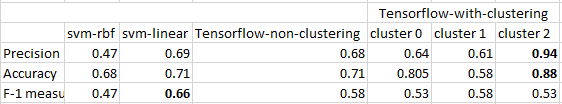
\includegraphics[width=0.5\textwidth]{Capture}
\caption{Result of different classifications}

\end{figure}







As we can see the result of each cluster in fig 2, the second cluster didn't perform as good as the other two. We don't know what are the tweets in this cluster, but if can improve the performance of it, the average of three clusters can get higher precision or accuracy.

\begin{figure}[h]
\centering
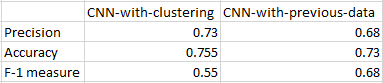
\includegraphics[width=0.5\textwidth]{Capture(4)}
\caption{Result of two Tensorflow models}
\end{figure}

In fig 3, we compare our model with the one training on both this year's and previous year's data. The Tensorflow with clustering means it only trains on this year's data. Tensorflow with previous data has both this year's and previous year's data. As we can see when the data grows, the F-1 score can easily beat the SVM. 

\begin{figure}[h]
\centering
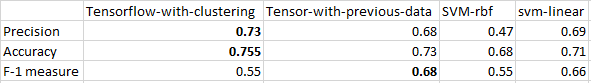
\includegraphics[width=0.5\textwidth]{Capture(5)}
\caption{Result of Tensorflow and SVM models with added data}
\end{figure}


To make it more convincing, we add previous year's data to svm model on both rbf and linear kernel.As we can see in fig 4, with more data, Tensorflow has a boost on F1-score, but the SVM models don't have much improvement. We conclude that, since our model has better performance than non-clustering one. And when data size grows, non-clustering Tensorflow model can beat normal classification models. Therefore, if we have more data which shares same topic scope of this year's data, our model will beat most of the classification models.


In a similar data set using the Semeval Twitter 2016 and the Twitter 2013 data for used by Vikrant et all 2016 , a direct comparison can be made between our model and the multilayer RNN used for binary classification. 
\begin{figure}[h]
\centering
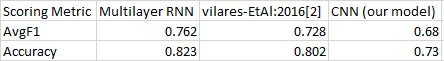
\includegraphics[width=0.5\textwidth]{Capture(6)}
\caption{A quick comparison of Multilayer RNN and CNN}
\end{figure}


\section{Conclusion}
In this paper, we proposed a model for sentiment analysis with pre-clustering processing by using pre-trained word embedding for initialization of Doc2Vec to make Twitter-specific topics easier to cluster. The tweets belong to one cluster carry the similar document vectors which derived from the GloVe word embedding specifically focusing on Twitter data. Then when finishing clustering, we feed all the tweets into Tensorflow neural network, which is good at find the boundary between tweets that are difficult to distinguish. By giving each Tensorflow model similar tweets, the fine line can be found individually on each cluster. When combined together, the overall performance is better than the model without pre-clustering. But the svm with linear kernel also has reasonable performance, especially the F1-score. Even though the first cluster and the last one have good performance in terms of precision and accuracy, the overall performance (shown in fig 3, second column) is not a great improvement, especially F1-score. But if we can give our model more tweets with the same topic scope collected for this year's data, we can claim that our model will have better performance than the baseline method we have. For the future work, we aim to distinguish which cluster has undesired results and then have more processing on that cluster. As we discussed, the second cluster has worst performance, and thus contaminate the overall result. By improving this one, we may be able to have larger improvement against our baseline methods.




% if have a single appendix:
%\appendix[Proof of the Zonklar Equations]
% or
%\appendix  % for no appendix heading
% do not use \section anymore after \appendix, only \section*
% is possibly needed

% use appendices with more than one appendix
% then use \section to start each appendix
% you must declare a \section before using any
% \subsection or using \label (\appendices by itself
% starts a section numbered zero.)
%


\appendices
\section*{appendices}
\begin{enumerate}
\item
The CNN model training in takes a lot of time especially if it is run on the CPU only mode. A model with about 10000 tweets in total for a two class classification took about 15 hours to train.
\item
One of the desired results of the experiments was getting the comparative performance of the word embeddings of bag of words, word2vec and the GloVE vectors but as the models took so much time to build and train we were not able to achieve the goal.
\item
In the current state we have not put in place any mechanism to correct the spellings in the tweets or to find the stems of the misspelled words in the tweets. In the same vein the emoticons in the current model are treated as word characters not in the vocabulary.


\end{enumerate}


% use section* for acknowledgement
%\section*{Acknowledgment}


%The authors would like to thank...


% Can use something like this to put references on a page
% by themselves when using endfloat and the captionsoff option.
\ifCLASSOPTIONcaptionsoff
  \newpage
\fi



% trigger a \newpage just before the given reference
% number - used to balance the columns on the last page
% adjust value as needed - may need to be readjusted if
% the document is modified later
%\IEEEtriggeratref{8}
% The "triggered" command can be changed if desired:
%\IEEEtriggercmd{\enlargethispage{-5in}}

% references section

% can use a bibliography generated by BibTeX as a .bbl file
% BibTeX documentation can be easily obtained at:
% http://www.ctan.org/tex-archive/biblio/bibtex/contrib/doc/
% The IEEEtran BibTeX style support page is at:
% http://www.michaelshell.org/tex/ieeetran/bibtex/
%\bibliographystyle{IEEEtran}
% argument is your BibTeX string definitions and bibliography database(s)
%\bibliography{IEEEabrv,../bib/paper}
%
% <OR> manually copy in the resultant .bbl file
% set second argument of \begin to the number of references
% (used to reserve space for the reference number labels box)
\begin{thebibliography}{1}

\bibitem{IEEEhowto:HLTCOE}
HLTCOE, JHU. "SemEval-2013 Task 2: Sentiment Analysis in Twitter." Atlanta, Georgia, USA 312 (2013).
\bibitem{IEEEhowto:Nakov}
Nakov, Preslav, et al. "SemEval-2016 task 4: Sentiment analysis in Twitter." Proceedings of the 10th international workshop on semantic evaluation (SemEval 2016), San Diego, US (forthcoming). 2016.
\bibitem{IEEEhowto:Kim}
Kim, Yoon. "Convolutional neural networks for sentence classification." arXiv preprint arXiv:1408.5882 (2014).
\bibitem{IEEEhowto:Zhang}
Zhang, Ye, and Byron Wallace. "A Sensitivity Analysis of (and Practitioners' Guide to) Convolutional Neural Networks for Sentence Classification." arXiv preprint arXiv:1510.03820 (2015).
\bibitem{IEEEhowto:Yadav}
Yadav, Vikrant. "thecerealkiller at SemEval-2016 Task 4: Deep learning based system for classifying sentiment of tweets on two point scale." Proceedings of SemEval (2016): 100-102.

\end{thebibliography}

% biography section
% 
% If you have an EPS/PDF photo (graphicx package needed) extra braces are
% needed around the contents of the optional argument to biography to prevent
% the LaTeX parser from getting confused when it sees the complicated
% \includegraphics command within an optional argument. (You could create
% your own custom macro containing the \includegraphics command to make things
% simpler here.)
%\begin{biography}[{\includegraphics[width=1in,height=1.25in,clip,keepaspectratio]{mshell}}]{Michael Shell}
% or if you just want to reserve a space for a photo:

\begin{IEEEbiography}[{\includegraphics[width=1in,height=1.25in,clip,keepaspectratio]{picture}}]{John Doe}
\blindtext
\end{IEEEbiography}

% You can push biographies down or up by placing
% a \vfill before or after them. The appropriate
% use of \vfill depends on what kind of text is
% on the last page and whether or not the columns
% are being equalized.

%\vfill

% Can be used to pull up biographies so that the bottom of the last one
% is flush with the other column.
%\enlargethispage{-5in}




% that's all folks
\end{document}


